\chapter{LP formulation}\label{chap:LP}

This chapter treats the current results on the LP relaxation of $k$-set packing. Section \ref{sec:StandardLP} starts with the results for the standard LP relaxation. Then Section \ref{sec:IntersectingLP} shows how to strengthen this LP and we prove a new bound for the integrality gap of this strengthened LP. Finally Section \ref{sec:SizeLP} presents how to decrease the size of this LP to a polynomial size. %Next we will treat some background on semidefinite programming and the Lov\'{a}sz Theta function. Then we will be able to show that there exists a polynomially sized SDP with the same improved integrality gap.

\section{The standard LP}\label{sec:StandardLP}

\paragraph{LP-formulation} View the set packing problem as the hypergraph matching problem like in Subsection \ref{subsec:Hypergraphs}. Introduce a variable $x_e$ for every hyperedge $e$ that indicates whether $e$ is included in the matching or not. The objective is to maximise $\displaystyle \sum_{e \in E} x_e$ such that every vertex is covered only once. For convenience we introduce the following notation.
%
\begin{equation*}
x(F) := \sum_{e \in F} x_e.
\end{equation*}
%
Hence the natural linear program looks like the following, denoted by \eqref{LP}. As before, $\delta(v)$ denotes the set of hyperedges incident to $v$.
%
%\begin{equation*}
%\begin{alignedat}{2}
%\text{max}  \quad & x(E) \ \\
%\text{s.t.} \quad & x\left(\delta(v)\right) \leq 1, & \quad & \forall v \in V \\
%                  & x_e \in \{0,1\},                & \quad & \forall e \in E
%\end{alignedat}
%\end{equation*}
%%
%The natural linear program thus becomes the following, denoted by \eqref{LP}.
%%
\begin{equation}\tag{LP}\label{LP}
\begin{alignedat}{2}
\text{max}  \quad & x(E) \ \\
\text{s.t.} \quad & x\left(\delta(v)\right) \leq 1, & \quad & \forall v \in V \\
                  & 0 \leq x_e \leq 1,              & \quad & \forall e \in E
\end{alignedat}
\end{equation}

\paragraph{Results} F\"{u}redi, Kahn and Seymour \cite{Seymour} have shown that the integrality gap of \eqref{LP} equals $k - 1 + \frac{1}{k}$ for $k$-uniform hypergraphs. They also show that in the case of a $k$-partite hypergraph the integrality gap equals $k-1$, but both proofs are non-algorithmic. Chan and Lau \cite{LapChiLau} gave an algorithmic proof of these facts and showed that the bounds are tight. Both results also extend to the weighted case.

\paragraph{Tight example} As a tight example for the non-$k$-partite case, consider the projective plane of order $k-1$. This is a hypergraph that is $k$-uniform (every hyperedge has cardinality $k$), $k$-regular (every vertex has degree $k$), in which every pair of hyperedges intersects in one vertex, and in which every pair of vertices is contained in exactly one hyperedge. Equivalently it is the Steiner system $S(2,k,k^2-k+1)$.
%intersecting (every two hyperedges intersect) and having $k^2-k+1$ hyperedges. %  projective plane of order $k$ is a set of points (vertices) and lines (edges) such that any two points determine a line, any two lines determine a point, every point has $k+1$ lines on it and every line contains $k+1$ points.
A projective plane of order $k$ exists if $k$ is a prime power and the conjecture that this is also a sufficient condition is a long standing open question. The projective plane of order 2 (thus corresponding to 3-set packing) is the well-known Fano plane. Figure \ref{fig:FanoPlane} depicts a Fano plane, where a hyperedge is represented by a line connecting three vertices.

%\begin{figure}
%        \centering
%        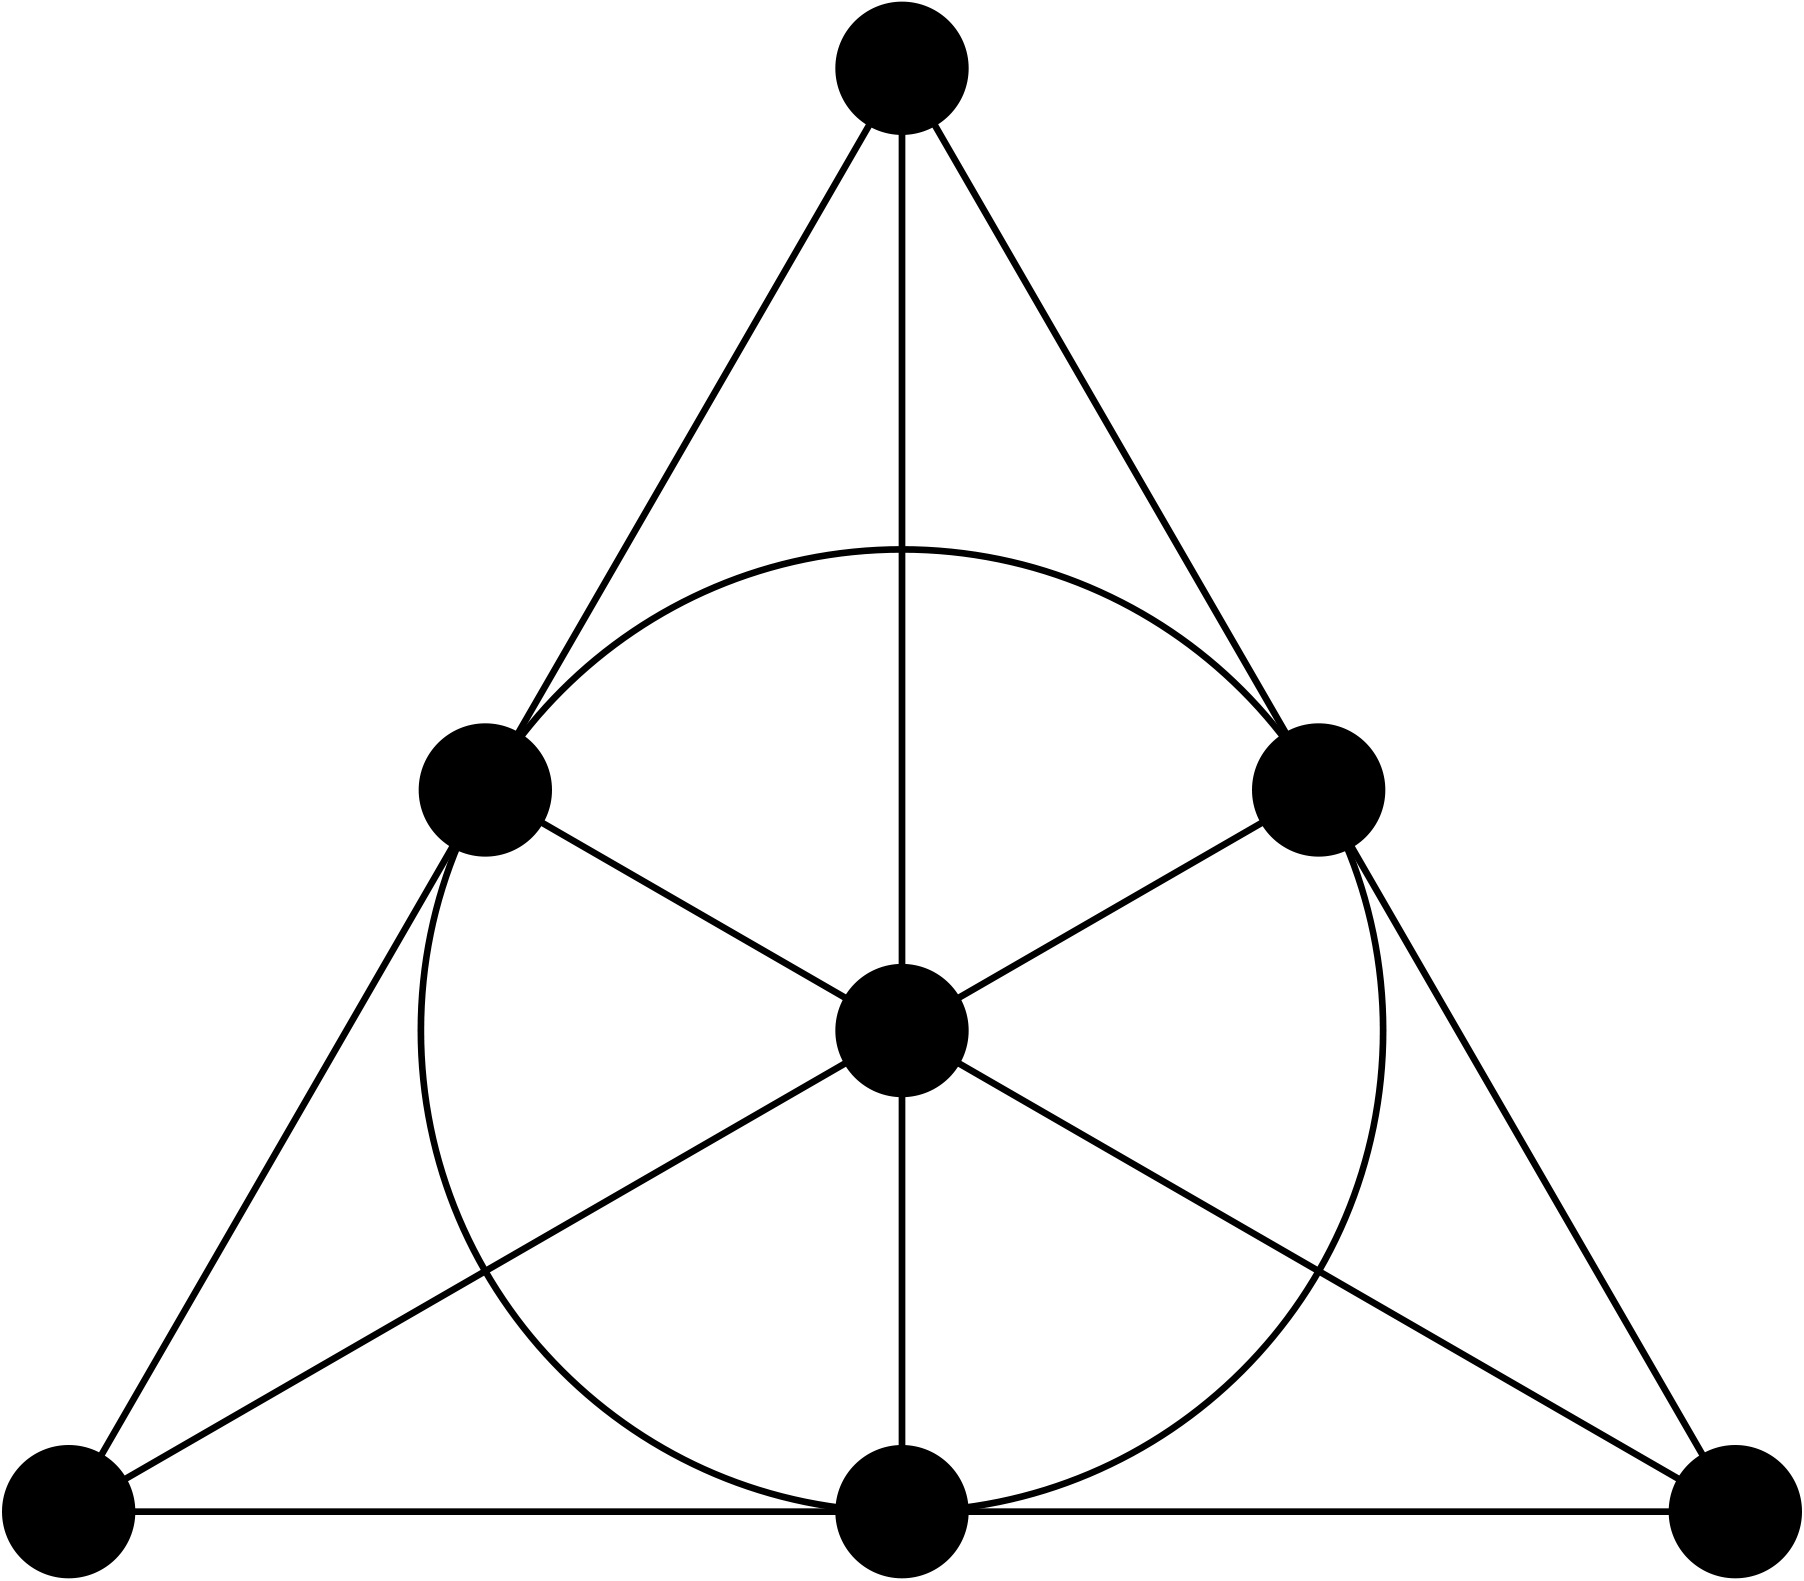
\includegraphics[width = 0.3 \textwidth]{Images/FanoPlane.jpg}
%        \caption{The Fano plane. A vertex is represented by a dot and a hyperedge is represented by a line connecting three dots.}
%        \label{fig:FanoPlane}
%\end{figure}

%\begin{figure}
%\centering
%\begin{tikzpicture}[scale=0.5]
%\vertex (a) at (0:0) {};
%\vertex (b) at (0:-10) {};
%\vertex (c) at (0:20) {};
%\vertex (d) at (9:5) {};
%\vertex (e) at (-9:5) {};
%\vertex (f) at (17:-10) {};
%\vertex (g) at (-17:-10) {};
%\path
%(a) edge (b)
%(a) edge (c)
%(a) edge (d)
%(a) edge (e)
%(a) edge (f)
%(a) edge (g)
%(b) edge (d)
%(b) edge (e)
%(b) edge (f)
%(b) edge (g)
%(c) edge (d)
%(c) edge (e)
%(d) edge (e)
%(d) edge (f)
%(d) edge (g)
%(e) edge (f)
%(e) edge (g);
%\end{tikzpicture}
%\caption{The Fano plane. A vertex is represented by a dot and a hyperedge is represented by a line connecting three dots.}
%\label{fig:FanoPlane}
%\end{figure}

\begin{figure}
\centering
\begin{tikzpicture}[main node/.style={circle,fill=black!10,draw,font=\sffamily\Large\bfseries}]
\node[main node] (centre) {\phantom{$_1$}};
\foreach \d/\lbl in {90/A, 210/B, 330/C} {
	\node[main node] (\lbl) at (\d:3.0cm) {\phantom{$_1$}};
}
\foreach \A/\B/\C in {A/B/C, B/C/A, A/C/B} {
	\node[main node] (\A\B) at ($(\A)!0.5!(\B)$) {\phantom{$_1$}};	
}
%\draw[edge] (centre) let \p1 = ($(AB)-(centre)$) in circle({veclen(\x1,\y1)});

\begin{pgfonlayer}{background}
\foreach \A/\B/\C in {A/B/C, B/C/A, A/C/B} {
\draw[edge] (\A) -- (\B);
	\draw[edge] (\A\B) -- (\C);
}
\draw[edge] (centre) let \p1 = ($(AB)-(centre)$) in circle({veclen(\x1,\y1)});
\end{pgfonlayer}

\end{tikzpicture}
\caption{The Fano plane. A hyperedge is represented by a line connecting three vertices.}
\label{fig:FanoPlane}
\end{figure}

%\begin{figure}
%\centering
%\begin{tikzpicture}
%\node[vertex] (centre) {};
%\foreach \d/\lbl in {90/A, 210/B, 330/C} {
%	\node[vertex] (\lbl) at (\d:0.8cm) {};
%}
%\foreach \A/\B/\C in {A/B/C, B/C/A, A/C/B} {
%	\node[vertex] (\A\B) at ($(\A)!0.5!(\B)$) {};
%	\draw (\A) -- (\B);
%	\draw (\A\B) -- (\C);
%}
%\draw (centre) let \p1 = ($(AB)-(centre)$) in circle({veclen(\x1,\y1)});
%\end{tikzpicture}
%\caption{The Fano plane. A vertex is represented by a dot and a hyperedge is represented by a line connecting three dots.}
%\label{fig:FanoPlane}
%\end{figure}

To see that the projective plane of order $k-1$ is a tight example, note that the integral solution to this $k$-set packing instance equals 1 as every hyperedge intersects every other hyperedge. But fractionally, it is possible to set $x_e = \frac{1}{k}$ for every hyperedge because the hypergraph is $k$-regular. This is a feasible solution to \eqref{LP} and since the hypergraph has $k^2-k+1$ hyperedges the integrality gap equals $\frac{1}{k}(k^2-k+1) = k - 1 + \frac{1}{k}$.

\section{Strengthening the LP formulation}\label{sec:IntersectingLP}

\subsection{The intersecting family LP}\label{subsec:IntersectingFamilyLP}

The LP formulation can be strengthened by adding extra local constraints. Call a family of hyperedges intersecting if every two of them overlap in at least one vertex. In the conflict graph of an instance, an intersecting family $\mathcal{F}$ would be a clique $F$. Obviously, from every intersecting family only one hyperedge can be picked. For every intersecting family thus an extra constraint can be added to obtain the following strengthened LP. Let $\mathcal{K}$ denote the collection of all intersecting families.
%
\begin{equation}\tag{Intersecting family LP}
\begin{alignedat}{2}
\text{max}  \quad & x(E) \ \\
\text{s.t.} \quad & x\left(\delta(v)\right) \leq 1, & \quad & \forall v \in V \\
            \quad & x\left(K\right) \leq 1,         & \quad & \forall K \in \mathcal{K} \\
                  & 0 \leq x_e \leq 1,              & \quad & \forall e \in E
\end{alignedat}
\end{equation}
%
This is called the interesting family LP. Note that this LP in general has exponentially many constraints and hence it is not solvable in polynomial time. In Section \ref{sec:SizeLP} we will show that for each $k$ the LP can be rewritten into an LP with a number of constraints that is polynomial in $n$. In \cite{LapChiLau}, they proved the following theorem about this intersecting family LP.
%
\begin{theorem}\label{thm:LPk+1/2}
(\cite[Theorem 4.1]{LapChiLau}) The ratio between any LP solution to the intersecting family LP and any 2-locally optimal solution is at most $\frac{k+1}{2}$. Thus the integrality gap of the intersecting family LP is at most $\frac{k+1}{2}$.
\end{theorem}
%
We omit the proof, because we will show an improved bound in Theorem \ref{thm:IntegralityGap2}. In order to proof this, the lemmas from \cite{BermanMIS} treated in the next subsections are necessary.

\subsection{A lemma on multigraphs}\label{subsec:lemma1}

\begin{lemma}\label{lem:BermanMIS1}
(\cite[Lemma 3.1]{BermanMIS}) Assume that every vertex in a multigraph\footnote{A multigraph is a graph where multiple edges and loops are allowed.} $G = (V,E)$ has degree at least 3. Then every vertex $v \in V$ belongs to a connected induced subgraph $G[X]$ with strictly more edges than vertices, of at most $4 \log_2 n - 1$ vertices.
\end{lemma}
%
\begin{proof}
This is a slightly more detailed proof than in \cite{BermanMIS}. Let $G = (V,E)$ be a multigraph where every vertex has degree at least 3 and let $v \in V$ be an arbitrary vertex. Consider a breadth-first search tree $T$ of $G$ rooted at $v$. The distance of a vertex in $T$ is the length of the shortest path from the vertex to $v$.

Let $m > 0$ and suppose every vertex in $T$ at a distance less than $m$ has at least two children. Then $T$ has at least $2^m$ vertices. Since $T$ has $n$ vertices, $m \leq \log_2 n$. Since $v$ has degree at least 3, in fact $m < \log_2 n$. This implies that there must be a vertex $u$ at a distance of at most $\log_2 n - 1$ having at most one child.

Since $u$ has at least degree 3 but at most one child, one of the edges incident to $u$ in $T$ must be a cross edge, a loop or a multiple edge. Let's denote this edge by $e = \{u,w\}$, where possibly $w = u$. Then the tree paths from $v$ to $u$ and from $v$ to $w$ together with the edge $e$ form an induced subgraph $G[Y]$ of at least as many edges as vertices, and this induced subgraph has at most $2 \log_2 n$ vertices.

If the number of edges in $G[Y]$ is already strictly larger than the number of vertices in $G[Y]$, then the proof is finished. Otherwise the number of edges equals the number of vertices. In this case, shrink $G[Y]$ to one single vertex $y$. In this modified graph $G'$, every vertex still has degree at least 3. Therefore $G'$ contains another induced subgraph induced by some $Z\cup\{y\}$ with at least as many edges as vertices, of size at most $2 \log_2 n$. But then $G[Y] \cup G[Z]$ contains strictly more edges than vertices in $G$ and its size is at most $4 \log_2 n - 1$, because $y$ is not a vertex in $G$. So $G[Y \cup Z]$ is an induced subgraph of $G$ that satisfies the required properties, as $G[Y \cup Z]$ has at least as many edges as $G[Y] \cup G[Z]$. %Note that $G[Y] \cup G[Z]$ has strictly more edges than vertices because the pseudo-vertex $y$ does not count anymore.
\end{proof}

\subsection{Another lemma on multigraphs}\label{subsec:lemma2}

Using this lemma following lemma can be proved, which is the one really needed for Theorem \ref{thm:IntegralityGap2}.
%
\begin{lemma}\label{lem:BermanMIS2}
(\cite[Lemma 3.2]{BermanMIS}) For any integer $h \geq 1$, any undirected multigraph $G = (V,E)$ with $|E| \geq \frac{h+1}{h} |V|$ contains a set $X$ of less than $4 h \log_2 n$ vertices, such that in $G[X]$ there are more edges than vertices.
\end{lemma}
%
\begin{proof}
Also this is a slightly more detailed proof than in \cite{BermanMIS}. Let $h$ be any positive integer. For convenience, for any undirected multigraph $H = (V(H),E(H))$ denote $|V(H)| = V_H$, $|E(H)| = E_H$. $H$ is said to satisfy Property $(*)$ if $E_H \geq \frac{h+1}{h} V_H$. Given a set of vertices $U$ in a multigraph $H$, denote $V_U := V_{H[U]}$, $E_U := E_{H[U]}$. $U$ is said to satisfy Property $(*)$ if its induced subgraph $H[U]$ satisfies Property $(*)$.

Let $G = (V,E)$ be an undirected multigraph that satisfies Property $(*)$, so $|E| \geq \frac{h+1}{h} |V|$. We need to show that $T$ contains a set $X$ of less than $4h \log_2 n$ vertices such that in $G[X]$ there are more edges than vertices.

Let $U \subseteq V$ be the smallest set of vertices in $G$ that satisfies Property $(*)$. Because $U$ is a minimal set, $G[U]$ cannot have a vertex $u$ of degree 1: otherwise $U \setminus \{u\}$ would be a smaller set satisfying Property $(*)$.

Now consider a maximal chain of degree 2 vertices $C$ in $G[U]$ and denote the two vertices adjacent to $C$, its endpoints in $G[U] \setminus C$, by $x$ and $y$. First we show that $C$ has less than $h$ vertices. Assume the contrary and suppose $C$ has exactly $h$ vertices. We claim that $U \setminus C$ is a smaller set of vertices that satisfies Property $(*)$ which is a contradiction. Note that $E_{U \setminus C} = E_U - h - 1$ because $G[C]$ contains $h-1$ edges and is connected to the rest of $U$ by 2 other edges. Also $V_{U \setminus C} = V_U - h$. So we need to show that $E_U - h - 1 \geq \frac{h+1}{h} (V_U - h)$. But this is true: subtract $h+1$ on both sides from the known fact that $E_U \geq \frac{h+1}{h} V_U$ to get to this equation.
%To show this, start with the given fact that $E_U \geq \frac{h+1}{h} V_U$. Now subtract $h+1$ on both sides to obtain the equivalent inequality $E_U - h - 1 \geq \frac{h+1}{h} V_U - (h+1)$. We write $h+1 = \frac{h+1}{h} \cdot h$ for the last term to write $E_U - h - 1 \geq \frac{h+1}{h} V_U - \frac{h+1}{h} \cdot h$. We can write this as $E_U - h - 1 \geq \frac{h+1}{h} (V_U - h)$, which is what we wanted to show.
So if $C$ contains $h$ vertices, $U$ is not the smallest set of vertices satisfying Property $(*)$, which is a contradiction. Note that the argument still holds if $C$ has $p > h$ vertices: then on the left-hand side $p+1$ is subtracted while on the right-hand side $\frac{h+1}{h}p = p + \frac{p}{h} > p+1$ is subtracted, so the left-hand side is indeed still larger than the right-hand side. We conclude that $C$ has strictly less than $h$ vertices.

Now modify the graph $G[U]$. Replace every maximal chain of degree 2 vertices $C$ by a single edge connecting its endpoints $x$ and $y$. Since any two such chains do not intersect (except possibly at their endpoints), every such chain is replaced independently from another. Denote the resulting graph, obtained from $G[U]$ by contracting all such chains, by $G'$. Then $G'$ does not have any vertices of degree 2 as they are all contracted.

%Now consider a chain of degree 2 nodes $\{v_1, \ldots, v_p\}$ in $G[U]$ and denote its endpoints by $x$ and $y$ (so $x$ is adjacent to $v_1$ and $y$ is adjacent to $v_p$). Any such chain of degree 2 nodes, together with its endpoints, has $p+1$ edges and $p+2$ vertices, and hence less edges than vertices. We can therefore replace every maximal such chain with a single edge connecting $x$ and $y$. Since any two such maximal chains do not intersect (except possibly at their endpoints), we can replace every maximal such chain independently from another. Denote the resulting graph, obtained from $G[U]$ by these contractions, by $G'$. Then $G'$ does not have any vertices of degree 2.

Therefore all vertices in $G'$ have degree at least 3, and Lemma \ref{lem:BermanMIS1} applies. Hence $G'$ contains some induced subgraph $G'[X']$ of size $m \leq 4 \log_2 n - 1$ with strictly more edges than vertices. Now select $m+1$ edges in $G'[X']$ and replace the edges that were chains in $G[U]$ by their respective chains of degree 2 vertices. Denote the resulting graph, obtained from $m+1$ edges from $G'[X']$ by expanding the chains, by $G[X]$ (note that $G[X]$ is indeed an induced subgraph of $G$ so this notation is valid).

Note that in the expanding of the chains, at most $m+1$ chains are expanded and every chain has size less than $h$. So $G[X]$ has in total at most $m + (m+1)(h-1) = (m+1)h - 1$ vertices. As $m \leq 4 \log_2 n - 1$ we see that $V_X = (m+1)h - 1 < 4 h \log_2 n$ vertices and the proof is complete.
\end{proof}
%
The following lemma is an immediate consequence.
%
\begin{lemma}\label{lem:BermanMIS3}
(Special case of Lemma \ref{lem:BermanMIS2}) Let $\varepsilon > 0$. If in an undirected multigraph $G = (V,E)$ there is no subset of vertices $X$ of size at most $4 (1 + \frac{1}{\varepsilon}) \log_2 n$ such that in $G[X]$ there are more edges than vertices, then $|E| \leq (1 + \varepsilon) |V|$.
\end{lemma}

\subsection{A new bound on the integrality gap}\label{subsec:TheoremLP}

Using this last lemma, the following improved bound on the integrality gap of the intersecting family LP can be established.
%
\begin{theorem}\label{thm:IntegralityGap2}
Let $\varepsilon > 0$. The ratio between any LP solution to the intersecting family LP and any $4 ( 1 + \frac{1}{\varepsilon} ) \log_2 n$-locally optimal solution is at most $\frac{k}{3} + 1 + \varepsilon$. Thus the integrality gap of the intersecting family LP is at most $\frac{k}{3} + 1 + \varepsilon$. \textbf{[NOTE: see page iii]}
\end{theorem}
%
\begin{proof}
Let $M$ be a $4 ( 1 + \frac{1}{\varepsilon} ) \log_2 n$-locally optimal matching. Let $x$ be a feasible solution to the intersecting family LP, and let $\mathcal{F}$ be the set of hyperedges with $x_e > 0$. To prove the theorem it suffices to prove that $x(\mathcal{F}) \leq \left( \frac{k}{3} + 1 + \varepsilon \right) |M|$. Denote by $\mathcal{F}_1$, $\mathcal{F}_2$ and $\mathcal{F}_{3+}$ the subsets of $\mathcal{F}$ in which every hyperedge in intersects exactly one, exactly two or at least three hyperedges in $M$, respectively.

Note that $M$ is in particular a 1-local and a 2-locally optimal matching. Since $M$ is a 1-locally optimal matching, each hyperedge $e$ in $\mathcal{F}$ intersects at least one hyperedge in $M$: otherwise $M \cup \{e\}$ would be a larger matching. Hence $\mathcal{F} = \mathcal{F}_1 \cup \mathcal{F}_2 \cup \mathcal{F}_{3+}$. We will now proceed to bound $x(\mathcal{F}_1)$ and $x(\mathcal{F}_2)$ in terms of $|M|$.

Consider a hyperedge $e$ in $M$ and define $\mathcal{F}_1(e) := \left\{ f \in \mathcal{F}_1 \mid f \cap e \neq \emptyset \right\}$. Then $\mathcal{F}_1(e)$ is an intersecting family. For suppose this is false, then there are two disjoint hyperedges $f_1, f_2$ in $\mathcal{F}_1$. These are disjoint from all other hyperedges in $M \setminus \{e\}$ because $f_1, f_2 \in \mathcal{F}_1$. Therefore $M - e + f_1 + f_2$ is a larger matching than $M$, but this is in contradiction with the fact that $M$ is a 2-locally optimal matching. Hence $\mathcal{F}_1(e)$ is an intersecting family. Thus by the intersecting family constraint $x(\mathcal{F}_1(e)) \leq 1$. Now summing over all hyperedges $e \in M$ yields
%
\begin{equation}\label{F1}
x(\mathcal{F}_1) \leq |M|.
\end{equation}

For the purpose of the analysis of the bound on $x(\mathcal{F}_2)$, consider an auxiliary multigraph $H$ with a vertex for every set in $M$. Two vertices $m_1, m_2 \in M$ are adjacent in $H$ if and only if there is a set in $\mathcal{F}_2$ that intersects both sets corresponding to $m_1$ and $m_2$. Note that $H$ consists of exactly $|M|$ vertices and $|\mathcal{F}_2|$ edges, potentially some of them are parallel. By assumption, $M$ cannot be improved by a set of size at most $4 ( 1 + \frac{1}{\varepsilon} ) \log_2 n$. As an induced subgraph of $H$ with more edges than vertices constitutes an improving set, $H$ cannot contain an induced subgraph of size at most $4 ( 1 + \frac{1}{\varepsilon} ) \log_2 n$ with more edges than vertices. Hence, by Lemma~\ref{lem:BermanMIS3} we infer that $|E(H)| \leq |V(H)| (1 + \varepsilon)$. Consequently, $|\mathcal{F}_2| \leq (1 + \varepsilon) |M|$. As $x(\mathcal{F}_2) \leq |\mathcal{F}_2|$ it follows that
%
\begin{equation}\label{F2}
x(\mathcal{F}_2) \leq (1 + \varepsilon) |M|.
\end{equation}

Now that $x(\mathcal{F}_1)$ and $x(\mathcal{F}_2)$ are upper bounded in terms of $|M|$, the result follows easily. Note that there are $k|M|$ vertices in $M$. Then the degree constraint yields
%
\begin{align*}
k|M| & \geq x(\mathcal{F}_1) + 2 x(\mathcal{F}_2) + 3 x(\mathcal{F}_{3+}) \\
     & = 3 x(\mathcal{F}) - x(\mathcal{F}_2) - 2 x(\mathcal{F}_1).
\end{align*}
%
Now plug in the bound from \eqref{F1} and \eqref{F2} to find
%
\begin{equation*}
k|M| \geq 3 x(\mathcal{F}) - (1 + \varepsilon) |M| - 2 |M|,
\end{equation*}
%
which can be rewritten as
%
\begin{equation*}
x(\mathcal{F}) \leq \frac{k + 3 + \varepsilon}{3} |M| \leq \left( \frac{k}{3} + 1 + \varepsilon \right) |M|. \qedhere
\end{equation*}
\end{proof}

%For completeness, another way to finish the proof is by writing the following.
%%
%\begin{equation*}
%x(\mathcal{F}_{3+}) \leq \frac{k|M| - x(\mathcal{F}_2) - 2 x(\mathcal{F}_1)}{3}.
%\end{equation*}
%%
%Now plug in the bounds for $x(\mathcal{F}_1)$, $x(\mathcal{F}_2)$ and $x(\mathcal{F}_{3+})$ in the equation
%%
%\begin{equation*}
%x(\mathcal{F}) = x(\mathcal{F}_1) + x(\mathcal{F}_2) + x(\mathcal{F}_3),
%\end{equation*}
%%
%and rewrite to find an integrality gap bounded by $\frac{k}{3} + 1 + \varepsilon$.

%Where the results for the standard LP extend to the weighted case, the results for the intersecting family LP do not. This is for the same reason why the unweighted approximation algorithms for $k$-set packing do not easily generalize to the weighted case: the local search technique is relying crucially on cardinality. For example, $\mathcal{F}_1(e)$ as in the previous proof need not be an intersecting family in the weighted case: the objective function might increase when we add less sets than we remove. It is not obvious how to improve significantly on the integrality gap of the standard LP for weighted $k$-set packing.

\section{A polynomially sized LP}\label{sec:SizeLP}

A new bound on the integrality gap of the intersecting family LP has now been established, but the LP might have exponentially many constraints and thus not solvable in polynomial time. This section treats the result from \cite{LapChiLau} that for constant $k$ only a polynomial number of constraints can be added to the standard LP formulation such that every intersecting family has a fractional value of at most 1. To this end the definition of a kernel is needed. Intuitively, for an intersecting family $K$ its kernel is a subset $U$ of the vertices covered by $K$ such that all hyperedges restricted to $U$ still form an intersecting family. More formally, for each hyperedge $e$ define $e_U = e \cap U$, and for a collection of hyperedges $K$ define $K_U = \{ e_u \mid e \in K \}$. Then $U$ is a kernel for an intersecting family $K$ if $K_U$ is an intersecting family.

We proceed with the following result from \cite{OriginalKernel}.
%
\begin{lemma}\label{lem:OriginalKernel}
(\cite{OriginalKernel}) For every $k$ there exists an $f(k)$ such that for every $k$-uniform intersecting family $K$ there is a kernel $S$ of cardinality at most $f(k)$.
\end{lemma}
%
The point of this lemma that will be exploited is that the size of this kernel $f(k)$ is independent of $n$ or the number of vertices of the hypergraph. This was a well-studied topic and the interested reader may read \cite{Kernel1,Kernel2,Kernel3,Kernel5,Kernel6,Kernel4}.
%The theorem has been generalized in \cite{Kernel5} to $s$-wise intersecting sets rather than mutually intersecting sets. In this more general setting the existence of $(k)$ is also proved in \cite{Kernel6}. The first explicit bound for $f(k)$ was given in \cite{Kernel2} and the current best bound is $f(k) = \Theta \left( {2k \choose k} \right)$ \cite{Kernel4}. See also \cite{Kernel1} for more details. %We mention a slightly weaker bound of the same order in the following lemma with a nice combinatorial proof.
%The interested reader may read \cite[Theorem 8]{Kernel3} or \cite[Exercise 13.27]{BookLovasz} for a nice proof of a slightly weaker bound.
%
%\begin{lemma}\label{lem:KernelLovasz}
%(\cite[Theorem 8]{Kernel3} and \cite[Exercise 13.27]{BookLovasz}) For every $k$ there exists an $f(k)$ such that for every $k$-uniform intersecting family $K$ there is a kernel $S$ of cardinality at most $f(k)$, where
%%
%\begin{equation}
%f(k) \leq (2k-1) {{2k-3} \choose {k-1}}.
%\end{equation}
%\end{lemma}
%%
%\begin{proof}
%[TODO] [TODO: see photo on mobile phone]
%
%Let $(x_1, \ldots, x_n)$ be any ordering of $W$, then $W$ is a minimal set such that any two edges of $H_W$ meet ($|W|=p$). Then there is at most one point $x_i$ such that both $\{x_1, \ldots, d_i\}$ and $\{x_i, \ldots, x_p\}$ contain edges $E, E'$ of $H_W$ (clearly $E \cap E' = \{x_i\}$). For if $j \neq i$ and $\{x_1, \ldots, x_j\}$ contained $F$, $\{x_j, \ldots, x_p\}$ contained $F'$ ($F, F' \in E(H_W)$), then assuming, e.g. $i<j$ we would have $E \cup F' = \emptyset$, a contradiction. So if we carry out the counting for every ordering of $W$, we count at most $p!$ points.
%
%Now every element of $W$ is counted many times. In fact, if $x \in W$, then there are edges, $E, F \in E(H_W)$, such that $E \cap F = \{x\}$, by the minimality of $W$. Set $|E| = s$, $|F| = t$. Let us arrange the points of $E$, then put $x$, then put the points of $F$; finally ``stick in'' the remaining points arbitrarily. This can be done in
%%
%\begin{equation*}
%(t-1)! (s-1)! {p \choose {s+t-1}} (p-s-t+1)! = p! \frac{(s-1)! (t-1)!}{(s+t-1)!}
%\end{equation*}
%%
%ways. Now $s,t \leq k$, hence
%%
%\begin{equation*}
%\frac{(s+t-1)!} {(s-1)! (t-1)!} = s {{s+t-1} \choose {t-1}} \leq k {{2k-1} \choose {r-1}}.
%\end{equation*}
%%
%Also we can exchange the role of $E$ and $F$. Thus every point in $W$ is counted at least $\frac{2p!}{k {{2k-1} \choose {k-1}}}$ times. Hence the number of points in $W$ is at most
%%
%\begin{equation*}
%\frac{ p! } { \frac{ 2p!}{k {{2k-1} \choose {k-1}} } } = \frac{k}{2} {{2k-1} \choose {k-1}} = (2k-1) {{2k-3} \choose {k-1}}.
%\end{equation*}
%
%[TODO] [TODO: change this proof. Maybe move to appendix?]
%\end{proof}
%
Now we will repeat the result from \cite{LapChiLau} that shows how to apply this lemma to prove the following theorem, with our improved bound on the integrality gap.
%
\begin{theorem}\label{thm:LP2}
Let $\varepsilon > 0$. There is a polynomially sized LP for $k$-set packing with integrality gap at most $\frac{k}{3} + 1 + \varepsilon$. \textbf{[NOTE: see page iii]}
\end{theorem}
%
\begin{proof}
We will prove it is possible to find a polynomially sized LP that still captures all the constraints of the intersecting family LP. This immediately implies the LP has the claimed integrality gap by Theorem \ref{thm:IntegralityGap2}. We follow the proof from \cite{LapChiLau}.

Let $G = (V,E)$ be the hypergraph and create a variable $x_U$ for every subset $U \subseteq V$ that is a subset of some hyperedge $e \in E$. To enforce that $x_U$ represents the fractional value of $U$, add the constraint $x_U = \sum_{e \supseteq U} x_e$. Each new variable $U$ is a subset of some hyperedges in $G$, and $U$ is said to be contained in a subset $S$ if $U \subseteq S$.

Now enumerate all possible subsets $S \subseteq V$ with $|S| \leq f(k)$. For each such subset $S$, enumerate all possible intersecting families $K_S$ formed by the new variables contained in $S$. For each such intersecting family $K_S$ write the following kernel constraint.
%
\begin{equation*}
\sum_{U \in K_S} x_U \leq 1.
\end{equation*}
%
There are $\sum_{i=1}^{f(k)} {n \choose i} \leq n^{f(k) + 1}$ possible kernels. For each kernel $S$ with $|S| = t$ there are at most $2^t$ new variables contained in $S$, because there are at most $2^t$ subsets of $S$. Hence there are at most $2^{2^t}$ intersecting families $K_S$ induced in $S$, because there are at most $2^{2^t}$ hypergraphs in $S$. Every such intersecting family corresponds to one constraint, so there are no more than $n^{f(k)+1} 2^{2^{f(k)}}$ kernel constraints. So when $k$ is a constant this is a number polynomial in $n$.

By Lemma \ref{lem:OriginalKernel} each intersecting family has a kernel constraint and hence each intersecting family has at most a fractional value of 1. So indeed, the intersecting family LP can be rewritten into a polynomially sized LP for every constant $k$.
\end{proof} 